\section{Pixel based classification}\label{sec:pbclassif}

\subsection{Classification}\label{ssec:classification}

The SVM classification in application framework provides a supervised pixel-wise
classification chain based on learning from multiple images. It supports huge
images through streaming and multi-threading.
The classification chain performs a SVM training step based on the intensities
of each pixel as features. Please note that all the input images must have the
same number of bands to be comparable.

\subsubsection{Statistics estimation}
In order to make these features comparable between each images, the first step
is to estimate the input images statistics. These statistics will be used to
center and reduce the intensities (mean of 0 and standard deviation of 1) of
samples based on the vector data produced by the user. To do so, the
\application{ComputeImagesStatistics} tool can be used :

\begin{verbatim}
otbcli_ComputeImagesStatistics -il  list_of_input_images
                               -out statistics.xml
\end{verbatim}

This tool will compute each band mean, compute the standard deviation based on
pooled variance of each band and finally export them to an XML file.
The features statistics XML file will be an input of the following tools.

\subsubsection{Building the training data set}

As the chain is supervised, we need first to build a training set with
positive examples of different objects of interest. This can be done
with Monteverdi Vectorization module
(Fig.\ref{fig:vectoModuleDataSetCreation}).
These polygons must be save in OGR vector format supported
by GDAL like ESRI shapefile for example.

This operation will be reproduced on each image used as input of the training
function.

Please note that the positive examples in the vector data should have a ``Class``
field with a label value higher than 1 and coherent in each images.

\begin{figure}
  \center
  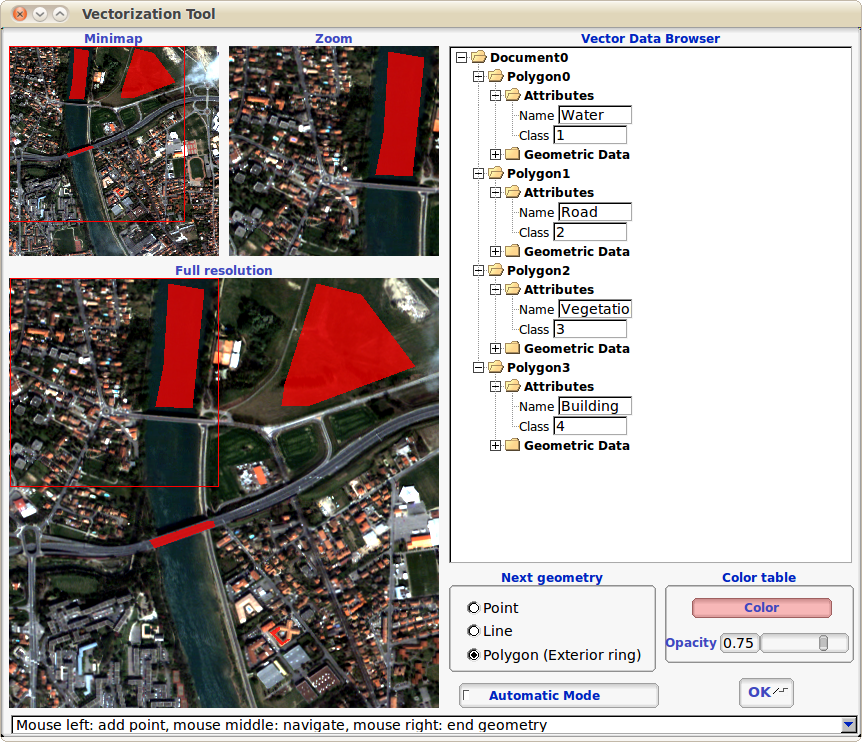
\includegraphics[width=1\textwidth]{../Art/MonteverdiImages/monteverdi_vectorization_module_for_classification.png}
  \itkcaption[GUI of the vectorization module with data for classification chain]{A training data set builded with the vectorization monteverdi module.}
  \label{fig:vectoModuleDataSetCreation}
\end{figure}

You can generate the vector data set with \qgis software for
example and save it in an OGR vector format supported by \gdal (ESRI
sphapefile for example). \app should be able to transform the
vector data into the image coordinate system.

\subsubsection{Performing the learning scheme}

Once images statistics have been estimated, the learning scheme is the following:
\begin{enumerate}
  \item For each input image:
  \begin{enumerate}
    \item Read the region of interest (ROI) inside the shapefile,
    \item Generate validation and training data within the ROI,
    \item Add vectors respectively to the training samples set and the validation
    samples set.
  \end{enumerate}
  \item Increase the size of the training samples set and balance it by
  generating new noisy samples from the previous ones,
  \item Perform the learning with this training set
  \item Estimate performances of the classifier on the validation samples set
  (confusion matrix, precision, recall and F-Score).
\end{enumerate}

These steps can be performed by the \application{TrainSVMImagesClassifier}
command-line using the following:

\begin{verbatim}
otbcli_TrainSVMImagesClassifier -io.imstat  images_statistics.xml
                                -io.il  list_of_input_images
                                -io.vd  list_of_positive_examples_shapefiles
                                -io.out model.svm
\end{verbatim}

Optionnal groups of parameters are also available (see application help for
more details):
\begin{itemize}
\item \verb?-elev? Handling of elevation (DEM or average elevation)
\item \verb?-sample? Group of parameters for sampling
\item \verb?-svm? Group of parameters for SVM
\end{itemize}

\subsubsection{Validating the classification model}
It is also possible to estimate the performance of the SVM model with a
new validation sample set and another image with the
\application{ValidateSVMImagesClassifier} application. It will compute
the global confusion matrix and precision, recall and F-score of each
class based on the \href{http://www.orfeo-toolbox.org/doxygen-current/classotb_1_1ConfusionMatrixCalculator.html}{ConfusionMatrixCalculator}
class.

\begin{verbatim}
otbcli_ValidateSVMImagesClassifier -imstat  images_statistics.xml
                                   -svm model.svm
                                   -il  input_image_list
                                   -vd  list_of_positive_examples_shapefiles
\end{verbatim}

You can save these results with the option -out output filename.
%You can also set a DEM repository (-dem) to keep the vectordata reprojection accurate.

\subsubsection{Using the classification model}
Once the classifier has been trained, one can apply the model to classify
pixel inside defined classes on a new image using the
\application{ImageSVMClassifier} application:

\begin{verbatim}
otbcli_ImageSVMClassifier -imstat  images_statistics.xml
                          -svm model.svm
                          -in  input_image
                          -out labeled_image
\end{verbatim}

You can set an input mask to limit the classification to the mask area with
value \textgreater 0.

\subsubsection{Fancy classification results}
\label{ssec:classificationcolormapping}
Color mapping can be used to apply color transformations on the final
graylevel label image. It allows to get an RGB classification map
by re-mapping the image values to be suitable for display purposes.
One can use the \application{ColorMapping} application. This tool will
replace each label with an 8-bits RGB color specificied in a mapping
file. The mapping file should look like this :

\begin{verbatim}
# Lines beginning with a # are ignored
1 255 0 0
\end{verbatim}

In the previous example, 1 is the label and 255 0 0 is a RGB color
(this one will be rendered as red). To use the mapping tool, enter
the following :

\begin{verbatim}
otbcli_ColorMapping -in  labeled_image
                    -out color_image
                    -method custom
                    -method.custom.lut  mapping_file
\end{verbatim}

Other look-up tables (LUT) are available : standard continuous LUT,
optimal LUT, and LUT computed over a support image.

\subsubsection{Example}

We take 4 classes: water, roads, vegetation and buildings with red roof.
Data is available in the OTB-Data
\href{http://hg.orfeo-toolbox.org/OTB-Data/file/0fed8f4f035c/Input/Classification}{repository}
and this image is produced with the commands inside this
\href{http://hg.orfeo-toolbox.org/OTB-Applications/file/3ce975605013/Testing/Classification/CMakeLists.txt}{file}.

\begin{figure}[!h]
  \center
  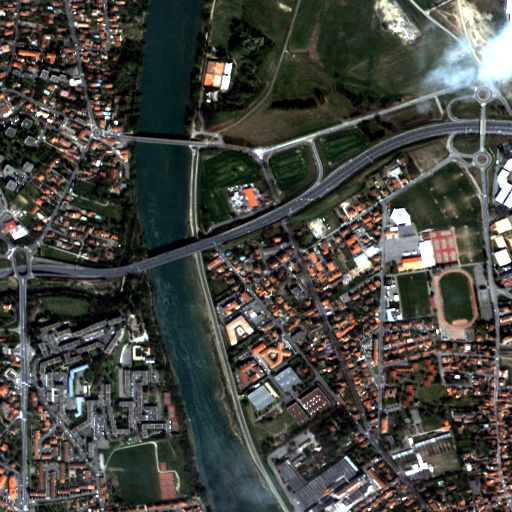
\includegraphics[width=0.3\textwidth]{../Art/MonteverdiImages/classification_chain_inputimage.jpg}
  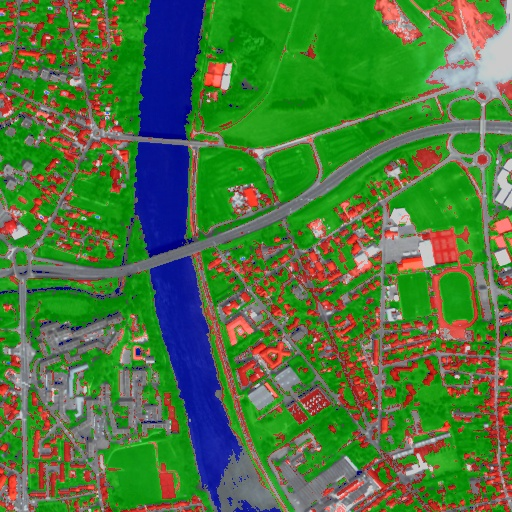
\includegraphics[width=0.3\textwidth]{../Art/MonteverdiImages/classification_chain_fancyclassif_fusion.jpg}
  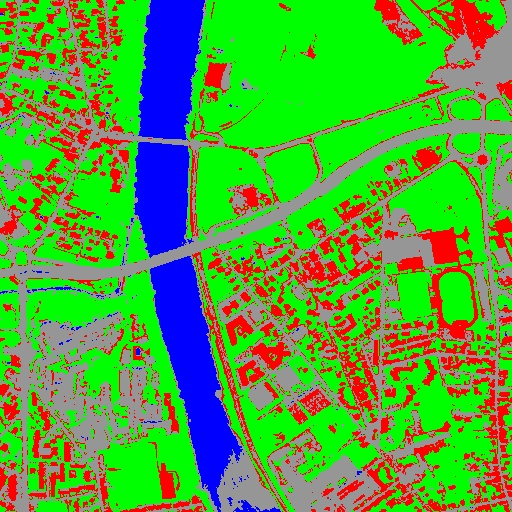
\includegraphics[width=0.3\textwidth]{../Art/MonteverdiImages/classification_chain_fancyclassif.jpg}
  \itkcaption[ExampleSVMClassif]{From left to right: Original image,
    result image with fusion (with monteverdi viewer) of original
    image and fancy classification and input image with fancy color
    classification from labeled image.}
  \label{fig:MeanShiftVectorImageFilter}
\end{figure}




\subsection{Fusion of classification maps}\label{ssec:fusionofclassifications}

After having processed several classifications of the same input image but from different models or methods (SVM,...),
it is possible to make a fusion of these classification maps with the \application{FusionOfClassifications} application which uses majority voting to handle
this fusion. The Fusion of Classifications generates a single more robust and precise classification map which combines the information extracted from the input
list of labeled images. 

\subsubsection{Majority voting for the fusion of classifications}

In the Majority Voting method implemented in the \application{FusionOfClassifications} application, the value of each output pixel is equal to the more frequent
class label of the same pixel in the input classification maps. However, it may happen that the more frequent class labels are not unique in individual pixels. In that case,
the undecided label is attributed to the output pixels.

The \application{FusionOfClassifications} application has the following input parameters :
\begin{itemize}
\item \verb?-il? list of input labeled classification images to fuse.
\item \verb?-out? the output labeled image resulting from the fusion of the input classification images.
\item \verb?-undecided? label for the undecided class (default value = 0).
\end{itemize}


The application can be used like this:
\begin{verbatim}
otbcli_FusionOfClassifications  -il         list_of_input_images
                                -out        OutputFusedClassificationImage
                                -undecided  10
\end{verbatim}
 

\subsubsection{Recommandations to properly use the fusion of classification maps}

In order to properly use the \application{FusionOfClassifications} application, some points should be considered. First, the \verb?list_of_input_images?
and \verb?OutputFusedClassificationImage? are single band labeled images, which means that the value of each pixel corresponds to the class label it belongs
to, and labels in each classification map must represent the same class. Secondly, the undecided label value must be different from existing labels in the input images in order to avoid any ambiguity in the interpretation of
the \verb?OutputFusedClassificationImage?.



\subsubsection{Example}

As an example of the \application{FusionOfClassifications} application, the fusion of the three input classification maps represented in
Fig. \ref{fig:ClassificationMapFusionApplication} leads to the classification map illustrated on the right in Fig. \ref{fig:ClassificationMapFusionApplication2}.
Thus, it appears that this fusion gives access to a more precise and robust classification map which highlight the more relevant classes among the three different input
classifications.


\begin{figure}[!h]
  \center
  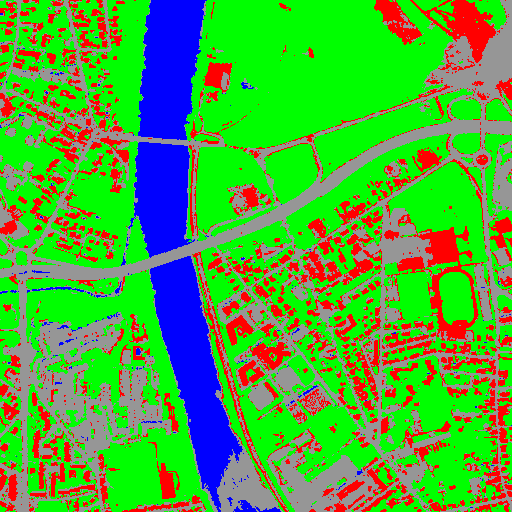
\includegraphics[width=0.3\textwidth]{../Art/MonteverdiImages/classification_chain_fancyclassif_CMR_input.png}
  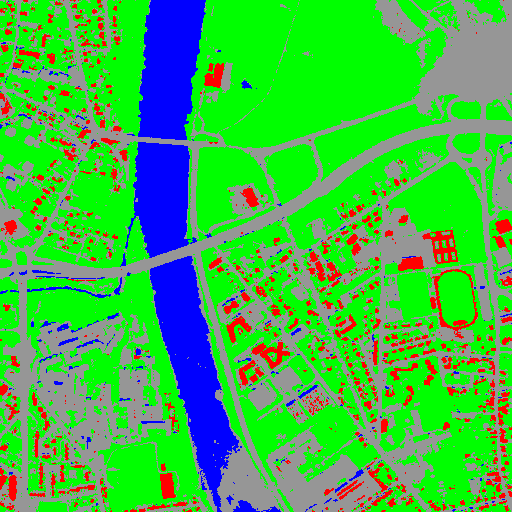
\includegraphics[width=0.3\textwidth]{../Art/MonteverdiImages/classification_chain_fancyclassif_CMR_input_2.png}
  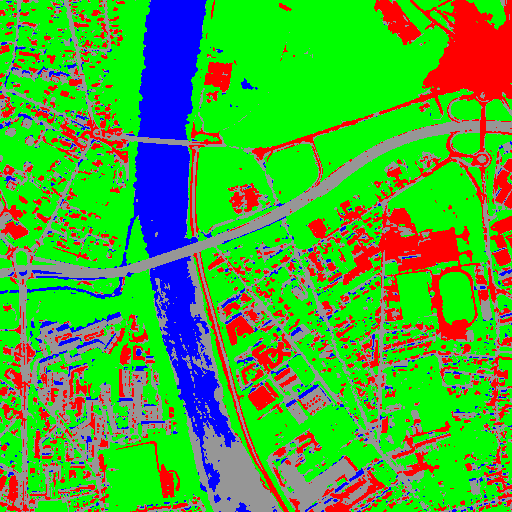
\includegraphics[width=0.3\textwidth]{../Art/MonteverdiImages/classification_chain_fancyclassif_CMR_input_3.png}
  \itkcaption[ExampleSVMClassifFusion]{Three fancy colored classified images to be fused, generated from 3 different SVM models.}
  \label{fig:ClassificationMapFusionApplication}
\end{figure}


\begin{figure}[!h]
  \center
  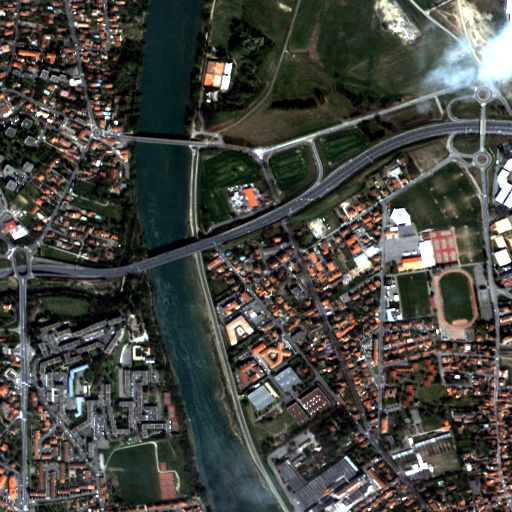
\includegraphics[width=0.3\textwidth]{../Art/MonteverdiImages/classification_chain_inputimage.jpg}
  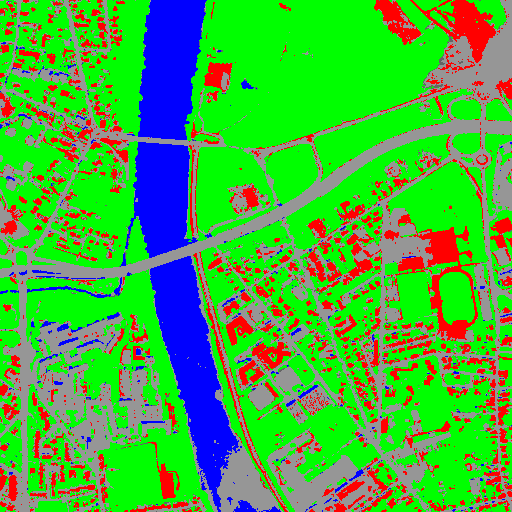
\includegraphics[width=0.3\textwidth]{../Art/MonteverdiImages/classification_chain_fancyclassif_CMR_Fusion_123.png}
  \itkcaption[ExampleSVMClassifFusion2]{From left to right: Original image, and fancy colored classified image obtained by a fusion of
  the 3 classification maps represented in Fig. \ref{fig:ClassificationMapFusionApplication}.}
  \label{fig:ClassificationMapFusionApplication2}
\end{figure}






\subsection{Majority voting based classification map regularization}\label{ssec:classificationmapregularization}

Resulting classification maps can be regularized in order to smoothen irregular classes. Such a regularization process
improves classification results by making more homogeneous areas which are easier to handle.

\subsubsection{Majority voting for the classification map regularization}

The \application{ClassificationMapRegularization} application performs a regularization of a labeled input image
based on the Majority Voting method in a specified ball shaped neighborhood. For each center pixel, Majority Voting takes the
more representative value of all the pixels identified by the structuring element and then sets the output center pixel
to this majority label value. The ball shaped neighborhood is identified by its radius expressed in pixels.


\subsubsection{Handling ambiguity and not classified pixels in the majority voting based regularization}

Since, the Majority Voting regularization may lead to not unique majority labels in the neighborhood, it is important to define
which behaviour the filter must have in this case. For this purpose, a Boolean parameter (called ip.suvbool) is used in the
\application{ClassificationMapRegularization} application to choose whether pixels with more than one majority class are set to
Undecided (true), or to their Original labels (false = default value).

Moreover, it may happen that pixels in the input image do not belong to any of the considered class. Such pixels are
assumed to belong to the NoData class, the label of which is specified as an input parameter for the regularization. Therefore,
those NoData input pixels are invariant and keep their NoData label in the output regularized image.
 
The \application{ClassificationMapRegularization} application has the following input parameters :
\begin{itemize}
\item \verb?-io.in? a labeled input image resulting from a previous classification process
\item \verb?-io.out? the output labeled image corresponding to the regularization of the input image
\item \verb?-ip.radius? an integer corresponding to the radius of the ball shaped structuring element (default value = 1 pixel)
\item \verb?-ip.suvbool? a Boolean number used to choose whether pixels with more than one majority class are set to Undecided (true),
or to their Original labels (false = default value). Please note that the Undecided value must be different from existing labels in the input image.
\item \verb?-ip.nodatalabel? label for the NoData class. Such input pixels keep their NoData label in the output image (default value = 0).
\item \verb?-ip.undecidedlabel? label for the Undecided class (default value = 0).
\end{itemize}


The application can be used like this:
\begin{verbatim}
otbcli_ClassificationMapRegularization  -io.in              InputLabeledImage
                                        -io.out             OutputLabeledImage
                                        -ip.radius          3
                                        -ip.suvbool         true
                                        -ip.nodatalabel     10
                                        -ip.undecidedlabel  7
\end{verbatim}
 

\subsubsection{Recommandations to properly use the majority voting based regularization}

In order to properly use the \application{ClassificationMapRegularization} application, some points should be considered.
First, both \verb?InputLabeledImage? and \verb?OutputLabeledImage? are single band labeled images, which means that the
value of each pixel corresponds to the class label it belongs to. The \verb?InputLabeledImage? is commonly an image generated
with a classification algorithm such as the SVM classification (see section \ref{ssec:classification}). Remark: both
\verb?InputLabeledImage? and \verb?OutputLabeledImage? are not necessarily of the same datatype. Secondly, if ip.suvbool == true,
the Undecided label value must be different from existing labels in the input labeled image in order to avoid any ambiguity in the
interpretation of the regularized \verb?OutputLabeledImage?. Finally, the structuring element radius must have a minimum value equal to 1 pixel,
which is its default value. Both NoData and Undecided labels have a default value equal to 0.


\subsubsection{Example}

Resulting from the \application{ColorMapping} application presented in section \ref{ssec:classificationcolormapping}, and illustrated in
Fig. \ref{fig:MeanShiftVectorImageFilter}, the Fig. \ref{fig:ClassificationMapRegularizationApplication} shows a regularization of a classification
map composed of 4 classes: water, roads, vegetation and buildings with red roof. The radius of the ball shaped structuring element is equal to 3 pixels,
which corresponds to a ball included in a 7 x 7 pixels square. Pixels with more than one majority class keep their original labels.

\begin{figure}[!h]
  \center
  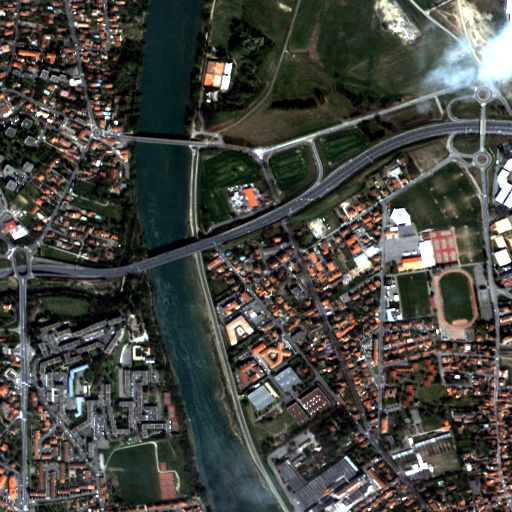
\includegraphics[width=0.3\textwidth]{../Art/MonteverdiImages/classification_chain_inputimage.jpg}
  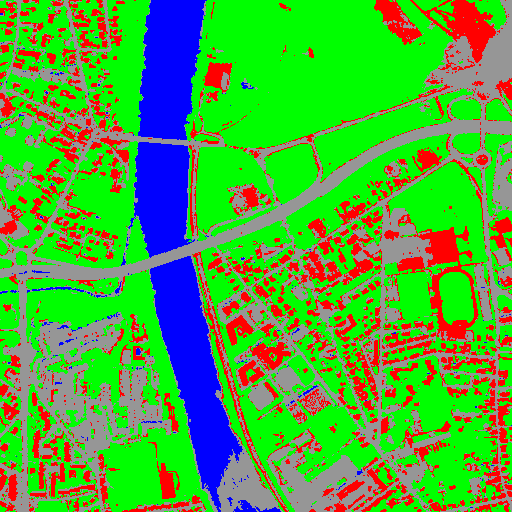
\includegraphics[width=0.3\textwidth]{../Art/MonteverdiImages/classification_chain_fancyclassif_CMR_input.png}
  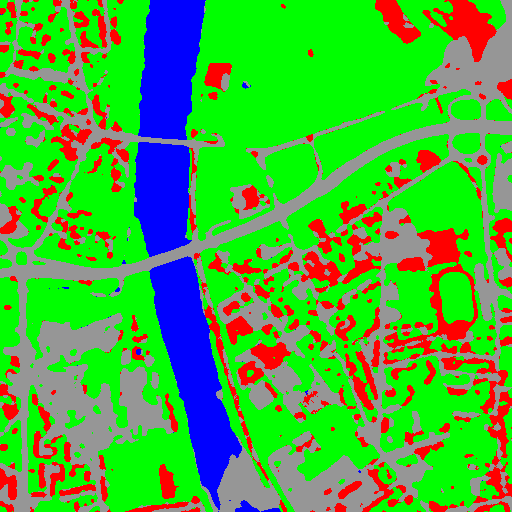
\includegraphics[width=0.3\textwidth]{../Art/MonteverdiImages/classification_chain_fancyclassif_CMR_3.png}
  \itkcaption[ExampleSVMClassifCMR]{From left to right: Original image, fancy colored classified image and regularized classification map with radius equal to 3 pixels.}
  \label{fig:ClassificationMapRegularizationApplication}
\end{figure}

